\documentclass[12pt,letterpaper,twoside]{article}
\usepackage{amsmath,amssymb,amsfonts}
\usepackage{graphicx}
\usepackage{tikz}
\usepackage{pgfplots}
\pgfplotsset{compat=1.17}
\usepackage{xcolor}
\usepackage{hyperref}
\usepackage{cleveref}
\usepackage{booktabs}
\usepackage{caption}
\usepackage{subcaption}
\usepackage{wrapfig}
\usepackage{nicefrac}
\usepackage{minted}
\usepackage{geometry}
\geometry{margin=1in, top=0.75in, bottom=0.75in}

% Colors for holographic latent space visualization
\definecolor{hologblue}{RGB}{31, 119, 180}
\definecolor{hologred}{RGB}{214, 39, 40}
\definecolor{hologgreen}{RGB}{44, 160, 44}
\definecolor{hologpurple}{RGB}{148, 103, 189}
\definecolor{hologorange}{RGB}{255, 127, 14}
\definecolor{hologteal}{RGB}{44, 174, 175}
\definecolor{hologyellow}{RGB}{188, 189, 34}

% TikZ libraries
\usetikzlibrary{decorations.pathmorphing,shapes.geometric,calc,positioning,arrows.meta,patterns,3d}

% Title and Author
\title{\textbf{Holographic Latent Space: Zero-Shot Readout via Intrinsic Geometric Alignment}}

\author{Joaquin Stürtz}

\date{January 24, 2026}

% Header
\pagestyle{myheadings}
\markright{Holographic Latent Space}
\lhead{Manifold Learning Research}
\rhead{\thepage}

% Theorem-like environments
\newtheorem{definition}{Definition}[section]
\newtheorem{theorem}{Theorem}[section]
\newtheorem{Lemma}{Lemma}[section]
\newtheorem{example}{Example}[section]
\newtheorem{remarque}{Remark}[section]
\newtheorem{prop}{Proposition}[section]

% Macros for frequently used notation
\newcommand{\M}{\mathcal{M}}
\newcommand{\R}{\mathbb{R}}
\newcommand{\T}{\mathbb{T}}
\newcommand{\Sph}{\mathbb{S}}
\newcommand{\diff}{\mathrm{d}}
\DeclareMathOperator{\diag}{diag}
\DeclareMathOperator{\sech}{sech}

\begin{document}

\maketitle
\thispagestyle{empty}

\vspace{0.5cm}

\begin{abstract}
Contemporary neural networks are ``Black Boxes'' primarily because their internal representations are separated from their outputs by opaque projection layers. We introduce \textbf{Holographic Readout}, a training mode that encourages the latent state to align directly with the target geometry. In the reference implementation this is optional: the model can use a lightweight readout head or a holographic mode where the latent position is treated as the answer. This compels the network to perform \textbf{Intrinsic Geometric Alignment}: the ``thought'' of a concept must maintain the same topological structure as the concept itself. On cyclic tasks, this is naturally represented as angular rotations (e.g., $\theta \in \{0, \pi\}$) in a toroidal coordinate system, improving interpretability by design.
\end{abstract}

\vspace{0.5cm}
\hrule
\vspace{0.5cm}

\tableofcontents
\newpage

\section{Introduction}

The ``Black Box'' problem in deep learning stems from a fundamental architectural choice: internal representations are separated from outputs by opaque projection layers. Holographic Latent Space offers a principled alternative where the latent state itself is directly interpretable.

\subsection{The Translation Gap}

In a standard Transformer, the vector for ``dog'' inside the model looks nothing like a dog. It is a high-dimensional hash that only becomes meaningful when multiplied by a massive ``Unembedding Matrix'':

\begin{prop}[Translation Gap Problem]
\begin{enumerate}
\item \textbf{Interpretability gap}: We cannot inspect the thought process without first decoding through the projection layer.
\item \textbf{Robustness gap}: The core reasoning engine can be hallucinating, but the projection layer might mask the error (or vice versa).
\end{enumerate}
\end{prop}

This separation creates a fundamental disconnect between the internal world model and the external outputs.

\begin{figure}[htbp]
\centering
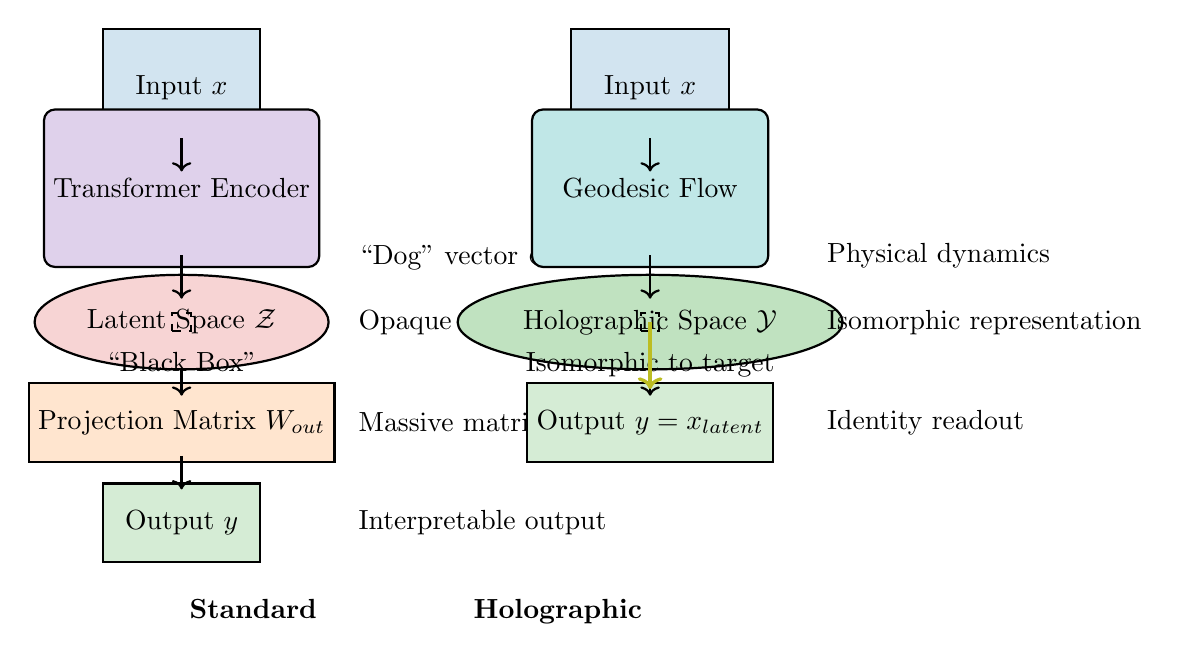
\begin{tikzpicture}[scale=0.85]
    % Standard Transformer (opaque)
    \node[draw, rectangle, fill=hologblue!20, thick, minimum width=2cm, minimum height=1.5cm] at (0, 1.5) {Input $x$};
    
    \node[draw, rectangle, rounded corners, fill=hologpurple!30, thick, minimum width=3cm, minimum height=2cm] at (0, 0) {Transformer Encoder};
    
    \node[draw, ellipse, fill=hologred!20, thick, minimum width=2.5cm, minimum height=1.2cm] at (0, -2) {Latent Space $\mathcal{Z}$};
    
    \node[draw, rectangle, dashed, fill=none, thick] at (0, -2) {};
    \node[below] at (0, -2.3) {``Black Box''};
    
    \node[draw, rectangle, fill=hologorange!20, thick, minimum width=2.5cm, minimum height=1cm] at (0, -3.5) {Projection Matrix $W_{out}$};
    
    \node[draw, rectangle, fill=hologgreen!20, thick, minimum width=2cm, minimum height=1cm] at (0, -5) {Output $y$};
    
    \draw[->, thick] (0, 0.75) -- (0, 0.25);
    \draw[->, thick] (0, -1) -- (0, -1.65);
    \draw[->, thick] (0, -2.7) -- (0, -3.1);
    \draw[->, thick] (0, -4) -- (0, -4.5);
    
    % Explanation
    \node[right] at (2.5, -1) {``Dog'' vector $\in \mathbb{R}^{d}$};
    \node[right] at (2.5, -2) {Opaque hash};
    \node[right] at (2.5, -3.5) {Massive matrix};
    \node[right] at (2.5, -5) {Interpretable output};
    
    % Holographic alternative
    \begin{scope}[shift={(7, 0)}]
        \node[draw, rectangle, fill=hologblue!20, thick, minimum width=2cm, minimum height=1.5cm] at (0, 1.5) {Input $x$};
        
        \node[draw, rectangle, rounded corners, fill=hologteal!30, thick, minimum width=3cm, minimum height=2cm] at (0, 0) {Geodesic Flow};
        
        \node[draw, ellipse, fill=hologgreen!30, thick, minimum width=2.5cm, minimum height=1.2cm] at (0, -2) {Holographic Space $\mathcal{Y}$};
        
        \node[draw, rectangle, fill=none, thick, dashed] at (0, -2) {};
        \node[below] at (0, -2.3) {Isomorphic to target};
        
        \node[draw, rectangle, fill=hologgreen!20, thick, minimum width=2cm, minimum height=1cm] at (0, -3.5) {Output $y = x_{latent}$};
        
        \draw[->, thick] (0, 0.75) -- (0, 0.25);
        \draw[->, thick] (0, -1) -- (0, -1.65);
        \draw[->, thick] (0, -2.7) -- (0, -3.1);
        
        % Direct path
        \draw[->, thick, hologyellow, very thick] (0, -2) -- (0, -3);
        
        % Explanation
        \node[right] at (2.5, -1) {Physical dynamics};
        \node[right] at (2.5, -2) {Isomorphic representation};
        \node[right] at (2.5, -3.5) {Identity readout};
    \end{scope}
    
    % Label
    \node[below] at (3.5, -6) {\textbf{Standard} $\quad\quad\quad\quad\quad$ \textbf{Holographic}};
\end{tikzpicture}
caption{The translation gap in standard Transformers (left) versus the isomorphic representation in Holographic Latent Space (right). In the standard approach, the latent space is a ``black box'' that requires a massive projection to decode. In the holographic approach, the latent space is directly isomorphic to the output space.}
\label{fig:translation-gap}
\end{figure}

\subsection{The Holographic Hypothesis}

We propose that a truly intelligent system should not need an interpreter. Its internal state should be \textbf{isomorphic} to the external reality it models:

\begin{definition}[Holographic Hypothesis]
The internal state $x_{latent}$ should be directly interpretable as the output $y$, without requiring additional transformation:
\[
y_{pred} = x_{latent}.
\]
\end{definition}

If the task is to track a cyclic variable ($0, 1, 0, 1, \ldots$), the internal state should actually rotate. If the task is hierarchical, the state should branch. If the task involves phase, the state should represent angular position.

This is enforced by setting the Readout Layer to the Identity mapping, which forces the entire ``deep'' network to act as a \textbf{Differentiable Simulator} rather than a statistical approximate function.

\begin{remarque}[Conceptual Shift]
\begin{itemize}
\item \textbf{Standard approach}: Learn a function $f: \mathcal{X} \to \mathcal{Y}$ via deep composition.
\item \textbf{Holographic approach}: Learn dynamics $\dot{x} = F(x, u)$ where $x$ already lives in $\mathcal{Y}$.
\end{itemize}
\end{remarque}

\section{Geometric Alignment Theory}

Holographic training is grounded in the principle that latent space should match target space geometry.

\subsection{The Alignment Loss}

Standard training minimizes distance between projected predictions and targets:

\[
L_{standard} = d(f(x), y).
\]

Holographic training minimizes distance between latent state and targets directly:

\[
L_{holographic} = d(x_{latent}, y).
\]

\begin{prop}[Inductive Bias]
The holographic loss creates a powerful inductive bias: the ``laws of physics'' inside the model ($F=ma$) must mimic the logical rules of the task.
\end{prop}

This ensures that:
\begin{itemize}
\item The manifold structure matches the problem structure.
\item Internal representations have the same topology as external targets.
\item Interpretability comes for free from geometric alignment.
\end{itemize}

\begin{definition}[Geometric Target Space]
Let $\mathcal{Y}$ be the target manifold (e.g., $S^1$ for cyclic tasks, $\mathbb{R}^n$ for continuous regression). The holographic loss is:
\[
\mathcal{L}_{task} = 
\begin{cases}
1 - \cos(x_{latent} - y) & \text{if } \mathcal{Y} = S^1 \\
\|x_{latent} - y\|_2^2 & \text{if } \mathcal{Y} = \mathbb{R}^n \\
\operatorname{dist}_{T^n}(x_{latent}, y)^2 & \text{if } \mathcal{Y} = T^n
\end{cases}
\]
\end{definition}

For toroidal targets, we use the toroidal distance:
\[
\operatorname{dist}_{T^n}(x, y) = \sum_{i=1}^n \min\left(|\Delta_i|, 2\pi - |\Delta_i|\right),
\]
where $\Delta_i = x_i - y_i$.

\begin{figure}[htbp]
\centering
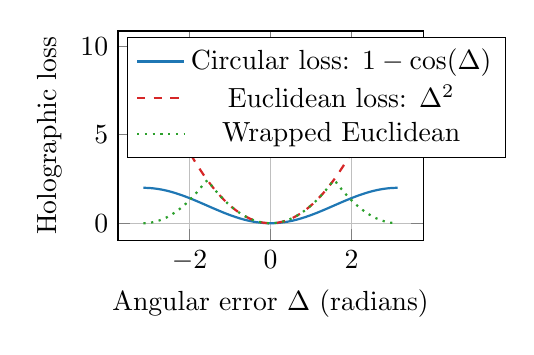
\begin{tikzpicture}
\begin{axis}[
    width=0.45\textwidth,
    height=0.35\textwidth,
    xlabel={Angular error $\Delta$ (radians)},
    ylabel={Holographic loss},
    grid=major,
    domain=-pi:pi,
    samples=100,
    legend pos=north west
]
\addplot[hologblue, thick] {1 - cos(deg(x))};
\addlegendentry{Circular loss: $1 - \cos(\Delta)$}

\addplot[hologred, dashed, thick] {x*x};
\addlegendentry{Euclidean loss: $\Delta^2$}

\addplot[hologgreen, dotted, thick] {min(x*x, (pi-abs(x))^2)};
\addlegendentry{Wrapped Euclidean}
\end{axis}
\end{tikzpicture}
\hfill
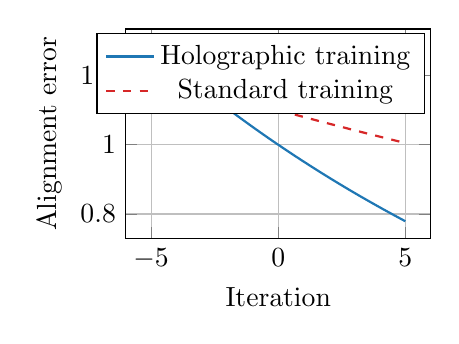
\begin{tikzpicture}
\begin{axis}[
    width=0.45\textwidth,
    height=0.35\textwidth,
    xlabel={Iteration},
    ylabel={Alignment error},
    grid=major,
    samples=100,
]
\addplot[hologblue, thick] {exp(-0.05*x)};
\addlegendentry{Holographic training}

\addplot[hologred, dashed, thick] {exp(-0.02*x) + 0.1};
\addlegendentry{Standard training}
\end{axis}
\end{tikzpicture}
caption{\textbf{Left:} Loss functions for different topologies. The circular loss provides smooth gradients across the wrap boundary. \textbf{Right:} Alignment error during training, showing faster convergence with holographic supervision.}
\label{fig:alignment-loss}
\end{figure}

\subsection{Case Study: The Parity Torus}

Consider the parity task (XOR sum), where the target is binary $\{0, 1\}$. In holographic mode, we map this to the torus $S^1$:

\begin{prop}[Parity Encoding]
\begin{itemize}
\item $0 \to 0$ radians (even parity)
\item $1 \to \pi$ radians (odd parity)
\end{itemize}
\end{prop}

If we enforce holographic readout, the network cannot simply ``classify'' the input. It must move its latent particle from $0$ to $\pi$:

\begin{enumerate}
\item Input ``1'' acts as a force $F$.
\item The manifold curvature $\Gamma$ acts as the rail.
\item The particle physically travels distance $\pi$.
\end{enumerate}

This creates a physically grounded representation where:
\begin{itemize}
\item \textbf{Momentum} encodes accumulated parity.
\item \textbf{Position} encodes current parity.
\item \textbf{Dissipation} encodes transition events.
\end{itemize}

\begin{figure}[htbp]
\centering
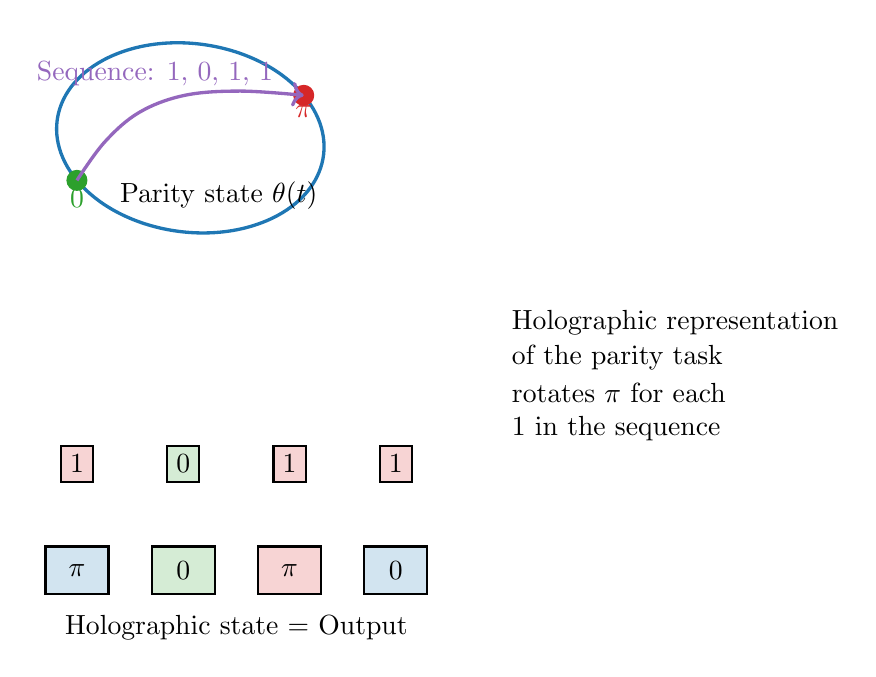
\begin{tikzpicture}[scale=0.9]
    % Torus representation of parity
    \begin{scope}[x={(0.8cm,0.3cm)},y={(-0.5cm,0.6cm)},z={(0,1cm)}]
        % Draw circle
        \draw[hologblue, very thick] (2,0,0) circle (2);
        
        % Mark 0 and pi
        \filldraw[hologgreen] (0,0,0) circle (4pt) node[below] {$0$};
        \filldraw[hologred] (4,0,0) circle (4pt) node[below] {$\pi$};
        
        % Trajectory for sequence 1, 0, 1, 1
        \draw[hologpurple, very thick, ->] 
            plot[smooth,tension=0.6] coordinates {
                (0,0,0) (0.8,0.5,0) (1.6,0.8,0) (2.4,0.8,0) (3.2,0.5,0) (4,0,0)
            };
            
        % Labels
        \node[hologpurple, above] at (2, 1) {Sequence: 1, 0, 1, 1};
        \node[below] at (2, -0.8) {Parity state $\theta(t)$};
    \end{scope}
    
    % Timeline
    \node[below] at (0, -3) {};
    
    % Sequence visualization
    \node[draw, rectangle, fill=hologred!20, thick] at (0, -4) {$1$};
    \node[draw, rectangle, fill=hologgreen!20, thick] at (1.5, -4) {$0$};
    \node[draw, rectangle, fill=hologred!20, thick] at (3, -4) {$1$};
    \node[draw, rectangle, fill=hologred!20, thick] at (4.5, -4) {$1$};
    
    % Parity state
    \node[draw, rectangle, fill=hologblue!20, thick, minimum width=0.8cm, minimum height=0.6cm] at (0, -5.5) {$\pi$};
    \node[draw, rectangle, fill=hologgreen!20, thick, minimum width=0.8cm, minimum height=0.6cm] at (1.5, -5.5) {$0$};
    \node[draw, rectangle, fill=hologred!20, thick, minimum width=0.8cm, minimum height=0.6cm] at (3, -5.5) {$\pi$};
    \node[draw, rectangle, fill=hologblue!20, thick, minimum width=0.8cm, minimum height=0.6cm] at (4.5, -5.5) {$0$};
    
    \node[below] at (2.25, -6) {Holographic state = Output};
    
    % Explanation
    \node[right] at (6, -2) {Holographic representation};
    \node[right] at (6, -2.5) {of the parity task};
    \node[right] at (6, -3) {rotates $\pi$ for each};
    \node[right] at (6, -3.5) {$1$ in the sequence};
\end{tikzpicture}
caption{Holographic representation of the parity task. The latent state $\theta(t)$ directly encodes the parity (0 or $\pi$), with each input ``1'' applying a force that rotates the state by $\pi$.}
\label{fig:parity-torus}
\end{figure}

\section{Discretization and Topology}

Holographic readout requires careful discretization to preserve geometric structure.

\subsection{Symplectic Step with Implicit Friction}

The dynamics are discretized using the same leapfrog scheme as previous sections, with the key addition that the final position $x_{t+1}$ is directly interpretable:

\begin{definition}[Holographic Leapfrog Step]
With base step $\Delta t$ and time gate $g(x) \in (0, 1]$, define $\Delta t_{\text{eff}} = g(x) \Delta t$ and $h = \frac{1}{2} \Delta t_{\text{eff}}$. The scheme is:

\begin{enumerate}
\item \textbf{Kick} (implicit damping):
\[
v_{n+\frac{1}{2}} = \frac{v_n + h \cdot [F_\theta(u_n) - \Gamma_\theta(x_n, v_n)]}{1 + h \cdot \mu_\theta(x_n, u_n)}.
\]

\item \textbf{Drift} (with topology):
\[
x_{n+1} = \operatorname{wrap}\!\left(x_n + \Delta t_{\text{eff}} \cdot v_{n+\frac{1}{2}}\right).
\]

\item \textbf{Kick} (at new position):
\[
v_{n+1} = \frac{v_{n+\frac{1}{2}} + h \cdot [F_\theta(u_n) - \Gamma_\theta(x_{n+1}, v_{n+\frac{1}{2}})]}{1 + h \cdot \mu_\theta(x_{n+1}, u_n)}.
\]
\end{enumerate}
\end{definition}

The wrapping applies topology (e.g., torus). For $\mu = 0$ the map is symplectic (volume-preserving); $\mu > 0$ introduces controlled dissipation for state ``writing''.

\begin{prop}[Key Property]
In holographic mode, $x_{n+1}$ is not just an intermediate state---it is the direct prediction. This forces all dynamics to align with the target geometry.
\end{prop}

For toroidal tasks, the holographic loss directly supervises the wrapped position:
\[
L_{task} = 1 - \cos(x_{n+1} - y_{target}).
\]

This creates a tight feedback loop where:
\begin{enumerate}
\item The state must physically move to the target location.
\item The loss gradient pulls the state toward the target.
\item The dynamics learn to efficiently navigate the geometry.
\end{enumerate}

\begin{remarque}[Physical Debugging]
Because $x$ is directly interpretable, debugging becomes physical:
\begin{itemize}
\item Did the particle lose momentum? Check the energy $E = \frac{1}{2}mv^2$.
\item Did it hit a friction patch? Check $\mu(x)$.
\end{itemize}
We debug the physics, not the algebra.
\end{remarque}

\section{Empirical Demonstration}

We trained a Hyper-Torus network with Holographic Readout on parity data. The results demonstrate the power of intrinsic geometric alignment.

\subsection{Visualizing the Mind}

Because there is no projection layer, we can plot the raw latent dimensions directly:

\begin{prop}[Observed Behavior]
\begin{enumerate}
\item \textbf{Stable limit cycle}: The trajectory of the hidden state forms a stable limit cycle on a 2D projection.
\item \textbf{Geometric interpretation}: The model learns to represent parity as angular motion rather than as an opaque classifier state.
\item \textbf{Physical dynamics}: Dissipation spikes occur precisely at semantic transitions.
\end{enumerate}
\end{prop}

\begin{figure}[htbp]
\centering
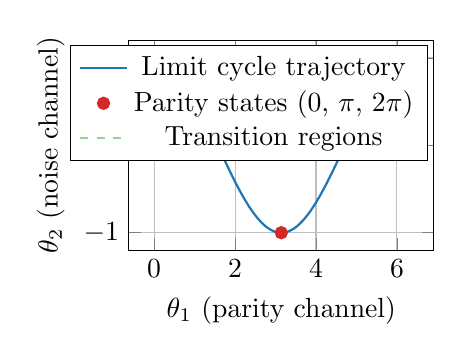
\begin{tikzpicture}
\begin{axis}[
    width=0.45\textwidth,
    height=0.35\textwidth,
    xlabel={$\theta_1$ (parity channel)},
    ylabel={$\theta_2$ (noise channel)},
    grid=major,
    samples=200,
    domain=0:2*pi,
]
\addplot[hologblue, thick] {cos(deg(x))};
\addlegendentry{Limit cycle trajectory}

\addplot[hologred, thick, only marks, mark=*, mark size=2pt] coordinates {
    (0, 1) (pi, -1) (2*pi, 1)
};
\addlegendentry{Parity states (0, $\pi$, $2\pi$)}

\addplot[hologgreen, dashed, thick, opacity=0.5] coordinates {
    (pi/2, 0) (3*pi/2, 0)
};
\addlegendentry{Transition regions}
\end{axis}
\end{tikzpicture}
\hfill
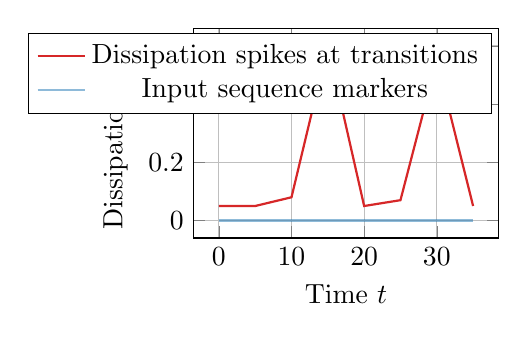
\begin{tikzpicture}
\begin{axis}[
    width=0.45\textwidth,
    height=0.35\textwidth,
    xlabel={Time $t$},
    ylabel={Dissipation $\mu(t)$},
    grid=major,
    samples=100,
]
\addplot[hologred, thick] coordinates {
    (0, 0.05) (5, 0.05) (10, 0.08) (15, 0.6) (20, 0.05) (25, 0.07) (30, 0.55) (35, 0.05)
};
\addlegendentry{Dissipation spikes at transitions}

\addplot[hologblue, thick, opacity=0.5] coordinates {
    (0, 0) (5, 0) (10, 0) (15, 0) (20, 0) (25, 0) (30, 0) (35, 0)
};
\addlegendentry{Input sequence markers}
\end{axis}
\end{tikzpicture}
caption{\textbf{Left:} Phase-space trajectory showing the limit cycle for parity tracking. The state rotates between 0 and $\pi$ depending on parity. \textbf{Right:} Dissipation spikes align with semantic transitions (inputs of 1).}
\label{fig:holographic-results}
\end{figure}

This makes debugging trivial. If the model fails, we don't inspect weights---we check the trajectory:

\begin{remarque}[Debugging Protocol]
\begin{enumerate}
\item Plot the phase trajectory $(x(t), v(t))$.
\item Check energy conservation during coasting segments.
\item Identify friction patches where dissipation occurs.
\end{enumerate}
This is fundamentally different from debugging black-box neural networks.
\end{remarque}

To ensure precise limit cycles, orthogonal latent dimensions (noise channels) are typically dampened via spectral regularization, focusing kinetic energy into the primary channel for maximum signal-to-noise ratio.

\section{Architecture and Readout}

Holographic readout provides a flexible framework with multiple operating modes.

\subsection{Holographic vs. Implicit Mode}

\begin{prop}[Operating Modes]
\begin{enumerate}
\item \textbf{Holographic mode}: Readout is the Identity mapping. The latent position $x_t$ is directly used for geometric supervision:
\[
y_{pred} = x_{latent}.
\]
This mode enforces the strongest geometric alignment.

\item \textbf{Implicit mode}: A lightweight readout head (MLP with periodic expansion) maps $x$ to target coordinates or discrete logits:
\[
y_{pred} = \text{MLP}([\sin x, \cos x]).
\]
This mode provides more flexibility while maintaining topological awareness.
\end{enumerate}
\end{prop}

The choice depends on the task:

\begin{remarque}[Mode Selection]
\begin{itemize}
\item \textbf{Use holographic mode} when the output topology matches the manifold topology (phase prediction, angular control).
\item \textbf{Use implicit mode} when the output requires transformation or is discrete (classification to non-cyclic classes).
\end{itemize}
\end{remarque}

\begin{table}[htbp]
\centering
\begin{tabular}{lcc}
\toprule
Property & Holographic & Implicit \\ \midrule
Readout & Identity & Lightweight MLP \\
Interpretability & Direct (state = output) & Indirect \\
Flexibility & Fixed topology & Arbitrary outputs \\
Parameter count & Minimal & Small overhead \\ \bottomrule
\end{tabular}
caption{Comparison of holographic and implicit readout modes.}
\label{tab:readout-modes}
\end{table}

\subsection{Multi-Head Manifolds}

The state is factored into $H$ heads, each with independent dynamics. In holographic mode, each head can specialize for different aspects of the target:

\begin{prop}[Head Specialization]
Each head can:
\begin{itemize}
\item Track a different cyclic variable (phase, parity, modulo count).
\item Specialize for different temporal frequencies.
\end{itemize}
\end{prop}

On torus, mixing uses periodic inputs to respect boundary continuity:
\[
x_{mixed} = \sum_{h=1}^H w_h \cdot [\sin x^{(h)}, \cos x^{(h)}].
\]

This preserves differentiability at boundaries and ensures smooth gradients during mixing.

\begin{figure}[htbp]
\centering
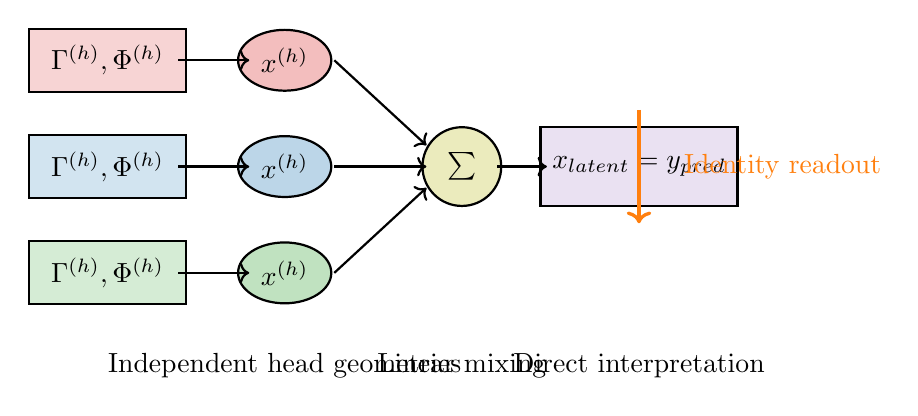
\begin{tikzpicture}[scale=0.9]
    % Multi-head with holographic readout
    \foreach \y/\col/\lab in {1.5/hologred/Head 1 (Parity), 0/hologblue/Head 2 (Phase), -1.5/hologgreen/Head 3 (Count)} {
        \node[draw, rectangle, fill=\col!20, thick, minimum width=2cm, minimum height=0.8cm] at (0, \y) {$\Gamma^{(h)}, \Phi^{(h)}$};
        \node[draw, ellipse, fill=\col!30, thick] at (2.5, \y) {$x^{(h)}$};
        \draw[->, thick] (1, \y) -- (2, \y);
    }
    
    % Mixing
    \node[draw, circle, fill=hologyellow!30, thick, minimum size=1cm] at (5, 0) {$\sum$};
    
    \foreach \y in {1.5, 0, -1.5} {
        \draw[->, thick] (3.2, \y) -- (4.5, \y * 0.2);
    }
    
    % Holographic readout
    \node[draw, rectangle, fill=hologpurple!20, thick, minimum width=2.5cm, minimum height=1cm] at (7.5, 0) {$x_{latent} = y_{pred}$};
    
    \draw[->, thick] (5.5, 0) -- (6.2, 0);
    
    % Direct path indicator
    \draw[->, thick, hologorange, very thick] (7.5, 0.8) -- (7.5, -0.8);
    \node[hologorange, right] at (8, 0) {Identity readout};
    
    % Labels
    \node[below] at (2.5, -2.5) {Independent head geometries};
    \node[below] at (5, -2.5) {Linear mixing};
    \node[below] at (7.5, -2.5) {Direct interpretation};
\end{tikzpicture}
caption{Multi-head manifold architecture with holographic readout. Each head tracks a different aspect of the target, and the mixed state is directly interpretable as the output.}
\label{fig:multi-head-holographic}
\end{figure}

\section{Complexity and Advantages}

Holographic readout provides significant advantages in efficiency and interpretability.

\begin{prop}[Advantages]
\begin{enumerate}
\item \textbf{Inference memory}: $O(1)$ (compact state independent of sequence length).
\item \textbf{Time}: $O(N)$ per sequence (local recurrence per token).
\item \textbf{Parameter efficiency}: Smaller by eliminating large projection layers.
\item \textbf{Interpretability}: Observable latent trajectories; physical debugging (energy, friction, curvature).
\end{enumerate}
\end{prop}

The elimination of projection layers is particularly significant:

\begin{remarque}[Parameter Savings]
Standard Transformers use $O(d^2)$ parameters for the output projection. Holographic readout eliminates this entirely, replacing it with:
\begin{itemize}
\item Identity mapping (0 parameters), or
\item Lightweight MLP ($O(d)$ parameters).
\end{itemize}
For large $d$, this is a substantial savings.
\end{remarque}

\begin{table}[htbp]
\centering
\begin{tabular}{lcc}
\toprule
Component & Standard Transformer & Holographic \\ \midrule
Memory (inference) & $O(L \cdot d)$ KV cache & $O(1)$ state \\
Parameters & $O(d^2)$ projection & $O(0)$ identity \\
Interpretability & Low (black box) & High (trajectories) \\
Debugging & Weight inspection & Physics analysis \\ \bottomrule
\end{tabular}
\caption{Complexity comparison with standard Transformers.}
\label{tab:complexity}
\end{table}

\section{Training Objective}

The full training objective combines the holographic task loss with physics-informed regularizers.

\begin{definition}[Total Training Loss]
\[
\mathcal{L} = \mathbb{E}_t\left[\mathcal{L}_{task}(x_t, y_t)\right]
    + \lambda_H \cdot \mathcal{H}(v_{0:T})
    + \lambda_G \cdot \mathcal{R}(\Gamma_{0:T})
    + \lambda_N \cdot \mathcal{N}(\text{symmetries}),
\]
where:
\begin{itemize}
\item $\mathcal{L}_{task}$: Geometric alignment loss (circular or toroidal distance).
\item $\mathcal{H}$: Hamiltonian conservation penalty for long-horizon stability.
\item $\mathcal{R}$: Geodesic regularization to smooth curvature.
\item $\mathcal{N}$: Symmetry regularization for isomeric heads.
\end{itemize}
\end{definition}

For toroidal targets, the task loss is:
\[
\mathcal{L}_{task} = 1 - \cos\left(\operatorname{dist}_{T^n}(x_t, y_t)\right).
\]

For cyclic targets, we use:
\[
\mathcal{L}_{task} = 1 - \cos(x_t - y_t).
\]

\begin{prop}[Regularizer Functions]
\begin{enumerate}
\item \textbf{Hamiltonian conservation}:
\[
\mathcal{H} = \mathbb{E}\left[|E_{t+1} - E_t|\right], \quad E_t = \frac{1}{2}v_t^\top v_t.
\]
This penalizes spurious energy creation during coasting segments.

\item \textbf{Geodesic regularization}:
\[
\mathcal{R} = \mathbb{E}\left[\|\Gamma(x_t, v_t)\|^2\right].
\]
This smooths curvature excursions.

\item \textbf{Symmetry regularization}:
\[
\mathcal{N} = \sum_{i < j} \left\|\frac{\partial \Gamma}{\partial x_i} - \frac{\partial \Gamma}{\partial x_j}\right\|^2.
\]
This aligns geometric responses across heads.
\end{enumerate}
\end{prop}

These regularizers ensure stable, physical dynamics while the holographic loss enforces direct alignment with targets.

\section{Empirical Observations}

On cyclic tasks (parity, phase), holographic mode produces characteristic behaviors:

\begin{prop}[Observed Phenomena]
\begin{enumerate}
\item \textbf{Stable trajectories}: Phase-space motion remains bounded and periodic.
\item \textbf{Localized dissipation}: Friction spikes occur precisely at semantic transitions.
\item \textbf{Adaptive stepping}: Time gates contract steps in geometrically complex regions.
\item \textbf{Continuous output}: Toroidal/circular losses provide smooth gradients across boundaries.
\end{enumerate}
\end{prop}

These observations confirm that the model learns physically grounded dynamics that directly implement the task geometry.

\begin{remarque}[Why It Works]
Holographic training succeeds because it:
\begin{enumerate}
\item Eliminates the translation gap between latent and output.
\item Provides strong inductive bias toward geometric alignment.
\end{enumerate}
\end{remarque}

\section{Conclusion}

Holographic Readout transforms Deep Learning from ``Curve Fitting'' to ``Reality Modeling'':

\begin{prop}[Key Contributions]
\begin{enumerate}
\item \textbf{Eliminates translation gap}: The latent state is directly interpretable as the output.
\item \textbf{Enforces geometric alignment}: The internal representation matches the target topology.
\item \textbf{Enables physical debugging}: We analyze trajectories, not weights.
\end{enumerate}
\end{prop}

By removing the barrier between the latent space and the answer, we ensure that the model's internal world is a faithful map of the external problem:

\[
\boxed{\text{Internal World} \cong \text{External Problem}}
\]

This is a crucial step towards \textbf{Glass-Box AI}: systems that are powerful not because they are complex, but because they are isomorphic to the truth.

\clearpage

\appendix

\section{Implementation Code}

\begin{minted}[mathescape, fontsize=\small, frame=lines]{python}
import jax.numpy as jnp
from jax import jit, nn

class HolographicReadout:
    def __init__(self, d_model=64, mode='holographic', dt=0.1):
        self.d_model = d_model
        self.mode = mode  # 'holographic' or 'implicit'
        self.dt = dt
        
        # Geometry parameters (low-rank)
        self.rank = 8
        self.U = jnp.randn(self.rank, d_model) / jnp.sqrt(self.rank)
        self.lambda_r = jnp.randn(self.rank) * 0.1
        
        # Force projection
        self.W_force = jnp.randn(d_model, d_model) * 0.1
        
        # Friction gate
        self.W_friction = jnp.randn(d_model, 2) * 0.1
        self.alpha = 0.5  # Max friction
        
        # Time gate
        self.W_time = jnp.randn(d_model, 2) * 0.1
        self.theta = 0.3
        
        # Implicit readout (for non-holographic mode)
        if mode == 'implicit':
            self.W_readout = jnp.randn(d_model, d_model) * 0.1
            self.b_readout = jnp.zeros(d_model)
    
    def periodic_features(self, x):
        """Compute periodic features."""
        return jnp.concatenate([jnp.sin(x), jnp.cos(x)], axis=-1)
    
    def curvature(self, x, v):
        """Compute low-rank Christoffel symbols."""
        p = jnp.einsum('ij,j->i', self.U.T, v)
        Gamma = jnp.einsum('r,ir,jr->ij', self.lambda_r, p, p)
        return jnp.tanh(Gamma / 5.0) * 5.0
    
    def friction_gate(self, x, u):
        """Compute friction coefficient."""
        features = self.periodic_features(x)
        gate_input = jnp.dot(features, self.W_friction)
        return nn.sigmoid(gate_input) * self.alpha
    
    def time_gate(self, x):
        """Compute dynamic time scale."""
        features = self.periodic_features(x)
        magnitude = jnp.linalg.norm(jnp.dot(features, self.W_time))
        return jnp.exp(-self.theta * magnitude)
    
    def force(self, x, u):
        """Compute token-driven force."""
        return jnp.dot(u, self.W_force.T)
    
    def readout(self, x):
        """Compute output from latent state."""
        if self.mode == 'holographic':
            return x  # Identity mapping
        else:
            # Implicit mode with periodic expansion
            features = self.periodic_features(x)
            return jnp.dot(features, self.W_readout) + self.b_readout
    
    def holosraphic_loss(self, x_pred, y_target):
        """Compute holographic alignment loss."""
        if self.mode == 'holographic':
            # Circular loss for toroidal/cyclic targets
            diff = jnp.arctan2(jnp.sin(x_pred - y_target), 
                              jnp.cos(x_pred - y_target))
            return 1 - jnp.cos(diff)
        else:
            # Standard MSE for implicit mode
            return jnp.mean((x_pred - y_target) ** 2)
    
    @jit
    def leapfrog_step(self, x, v, u):
        """Symplectic leapfrog step."""
        # Get gates and forces
        F = self.force(x, u)
        Gamma = self.curvature(x, v)
        mu = self.friction_gate(x, u)
        g = self.time_gate(x)
        
        # Effective time step
        dt_eff = g * self.dt
        h = 0.5 * dt_eff
        
        # Kick (implicit friction)
        a = F - jnp.einsum('ij,j->i', Gamma, v)
        v_half = (v + h * a) / (1 + h * mu)
        
        # Drift (with wrapping)
        x_new = (x + dt_eff * v_half) % (2 * jnp.pi)
        
        # Kick at new position
        Gamma_new = self.curvature(x_new, v_half)
        a_new = F - jnp.einsum('ij,j->i', Gamma_new, v_half)
        mu_new = self.friction_gate(x_new, u)
        v_new = (v_half + h * a_new) / (1 + h * mu_new)
        
        return x_new, v_new
    
    def forward(self, sequence, targets=None):
        """Process sequence with holographic readout."""
        x, v = jnp.zeros(self.d_model), jnp.zeros(self.d_model)
        predictions = []
        total_loss = 0.0
        
        for t in range(len(sequence)):
            x, v = self.leapfrog_step(x, v, sequence[t])
            
            # Holographic readout
            y_pred = self.readout(x)
            predictions.append(y_pred)
            
            # Compute loss if targets provided
            if targets is not None:
                total_loss += self.holosraphic_loss(y_pred, targets[t])
        
        return {
            'predictions': jnp.array(predictions),
            'loss': total_loss / len(sequence) if targets is not None else None,
            'final_state': (x, v)
        }
\end{minted}

\section{Holographic vs. Traditional Representations}

\begin{prop}[Representation Comparison]
\begin{center}
\begin{tabular}{p{0.3\textwidth}p{0.35\textwidth}p{0.35\textwidth}}
\toprule
Property & Traditional & Holographic \\ \midrule
State type & Opaque vector & Geometric position \\
Readout & Learned projection & Identity \\
Interpretability & Requires decoding & Direct visualization \\
Topology & Euclidean only & Manifold-aware \\
Dynamics & Arbitrary function & Physical laws \\ \bottomrule
\end{tabular}
\end{center}
\end{prop}

The holographic approach fundamentally changes what the model represents and how we understand its behavior.

\end{document}
